\documentclass[a4paper,12pt]{scrartcl}

\usepackage[utf8]{inputenc}
\usepackage[ngerman]{babel}
\usepackage{amsmath}
\usepackage[a4paper, left=3cm, right=2.5cm, top=2.5cm, bottom=3cm]{geometry}
\usepackage{graphicx}
\usepackage{csquotes}
\usepackage{hyperref}
\usepackage[figure]{hypcap}
\usepackage{listings}
\usepackage{xcolor}

\definecolor{codegreen}{rgb}{0,0.6,0}
\definecolor{codegray}{rgb}{0.5,0.5,0.5}
\definecolor{codepurple}{rgb}{0.58,0,0.82}
\definecolor{backcolour}{rgb}{0.95,0.95,0.92}

\lstdefinestyle{mystyle}{
    backgroundcolor=\color{backcolour},   
    commentstyle=\color{codegreen},
    keywordstyle=\color{magenta},
    numberstyle=\tiny\color{codegray},
    stringstyle=\color{codepurple},
    basicstyle=\ttfamily\footnotesize,
    breakatwhitespace=false,         
    breaklines=true,                 
    captionpos=b,                    
    keepspaces=true,                 
    numbers=left,                    
    numbersep=10pt,                  
    showspaces=false,                
    showstringspaces=false,
    showtabs=false,                  
    tabsize=2
}

\lstset{style=mystyle}

\usepackage{footnote}
\makesavenoteenv{table}
\makesavenoteenv{tabular}

\title {Ausarbeitung}
\author{Zoe Luca Günther}

\makeatletter
\def\@maketitle{%
  \newpage
  \null
  \vskip 15em%
  \begin{center}%
  \let \footnote \thanks
    {\LARGE \@title \par}%
    \vskip 1em%
    {\Large Ein Snake Spiel mit Darstellung über einen Raspberry Pi \par}%
    \vskip 5em%
    {\large
      \lineskip .5em%
      \begin{tabular}[t]{c}%
        \@author
      \end{tabular}\par}%
    \vskip 1em%
    {\large \@date}%
  \end{center}%
  \par
  \vskip 1.5em}
\makeatother

\begin{document}

\pagenumbering{Roman}
\maketitle
\newpage
\tableofcontents
\newpage
\listoffigures
\newpage
\pagenumbering{arabic}

\section{Einleitung}
% was habe ich in diesem projekt gemacht
In diesem Projekt habe ich ein Snake Spiel entwickelt. Hierbei ist das besondere, dass man dieses Snake Spiel über die Lagesensoren des Handys steuern kann. Man verbindet sich mit einer Website, geht in die Warteschlange rein und sobald man an der Reihe ist, wird man zur Spielsteuerung weitergeleitet [\ref{fig:main-menu}][\ref{fig:main-menu-queue}]. Am Anfang jedes Spiels wird ein kurzer Hinweis am Handy eingeblendet, welcher einem sagt, dass man das Handy vertikal und flach halten soll und die Bildschirmrotation deaktiviert werden sollte [\ref{fig:controller-hint-1}][\ref{fig:controller-hint-2}]. Dies ist wichtig, damit die Steuerung richtig funktioniert, da man um das Spiel zu steuern, lediglich sein Handy neigen muss. Um Das Spielerlebnis so gut wie möglich zu halten, muss das Handy flach und vertikal gehalten werden, da so die Steuerung am besten funktioniert, da diese sehr sensibel sein kann.
Um das Spielgeschehen zu sehen, wird ein Raspberry Pi mit einer 64x64 LED Matrix verwendet, worauf der Score und das Spiel dargestellt werden. Um das Spiel zu pausieren, klickt man lediglich auf seinem Handy auf den Pause Button [\ref{fig:controller}]. Dies geht jedoch nur, wenn man gerade an der Reihe ist. Um dies zu überprüfen, wird beim ersten betreten der Spiel Website ein Cookie gesetzt, worin die User ID steht. Jede ID ist unterschiedlich, um eine genaue Identifizierung zu ermöglichen.
Sollte sich ein Spieler für mehr als 20 Sekunden im Pause Status befinden, oder mehr als 20 Sekunden keine Bewegung mehr machen, wird das Spiel beendet und der nächste Spieler aus der Warteschlange kann spielen. Nachdem man sich selber als Schlange gefressen hat, oder man zu lange im Spiel war, wird man auf eine Game Over Seite weitergeleitet, wo der eigene Score eingeblendet wird [\ref{fig:gameover}].
% bilder als anhang

\section{Vorgehensweise}
% wie bin ich vorgegangen und welche tools habe ich benutzt
% erst in pygame das grundgerüst gemacht
% dann die api
% dann die darstellung auf dem raspi mit rpi rgb matrix api
% welche bibliothekene habe ich benutzt

Das Projekt wurde in verschiedene Unterpunkte eingeteilt, um die bestmögliche Implementierung sicherzustellen.


\subsection{Grundgerüst}
Das Grundgerüst besteht aus verschiedenen Klassen, welche für den Spielablauf essentiell sind. Folgende Klassen beinhaltet das Grundgerüst:

\newpage

\begin{table}
\centering
\begin{tabular}[!htb]{p{4cm}|p{10cm}}
Klassenname & Beschreibung \\
\hline
Player.py & Zuständig für die Bewegung des Spielers, des Überprüfens auf Kollision, das Score Handling und das Fressen von Futter \\
Logger.py & Ausgeben von Nachrichten in der Konsole zu Debug Zwecken. Es kann ein Prefix der Klasse Prefix.py angegeben werden \\
Playground.py & Handling des Spielfeld, setzen von Blöcken\footnote{Das Spielfeld besteht aus Blöcken, welche in einem 2d Array gespeichert sind} auf dem Spielfeld, setzen einer Random Futter Position, Prüfen ob das Spielfeld voll ist \\
Queue.py & Generelles Queue Handling (Spieler hinzufügen, entfernen aus Queue), Nächsten Spieler nehmen, UserId verifizieren\footnote{Überprüfen ob die UserId die nötige länge hat} \\
SnakeGame.py & Game Status setzen, Game starten / stoppen / pausieren, Game loop, game resetten, game over Handling \\
\end{tabular}
\caption{Grundgerüst Klassen}
\end{table}

\begin{table}
\centering
\begin{tabular}[!htb]{p{4cm}|p{10cm}}
Klassenname & Beschreibung \\
\hline
Direction.py & Richtungsangaben \\
GameStatus.py & Gamestatus mit Gamestatus Text \\
Message.py & Game over Nachrichten \\
PlaygroundTile.py & Spielfeld Blöcke (zum Beispiel Wand, Snake, Futter) \\
Prefix.py & Prefix zu Debug Zwecken \\
\end{tabular}
\caption{Enum Klassen}
\end{table}

Zum testen der Funktionalitäten, wurde das Spiel vorerst mithilfe der Bibliothek \textit{pygame} implementiert. Somit konnte das Spiel dargestellt werden, die Bewegungsabläufe getestet und der Spielablauf angepasst werden. Für den Gameloop wurde jedoch zu diesem Zeitpunkt die pygame eigenen Funktionen verwendet. Die Steuerung wurde vorerst über die Tastatur implementiert, da die spätere Steuerung über die Website mithilfe der API Schnittstelle funktioniert.

\subsection{Website}
\subsection{API Schnittstelle}
\subsection{Darstellung}


\section{Schwierigkeiten}
Die größte Schwierigkeit war, die API nicht zu unterbrechen, während das Spiel läuft. Es wurde \textit{multithreading} verwendet, um verschiedene Thread parallel laufen zu lassen. Somit laufen im fertigen Projekt der Thread für die Darstellung des Spiels auf dem Raspberry Pi, der Gameloop, die Überprüfung ob ein Spieler keine Inputs mehr macht und somit nicht mehr anwesend ist (AFK\footnote{away from keyboard, abwesend}) und die API Schnittstelle parallel. Es wurde versucht, einen neuen Prozess für die Darstellung auf dem Display zu verwenden, jedoch können live updates in einem separaten Prozess nicht mehr nachverfolgt werden, weshalb die Thread Variante verwendet worden ist. Die Thread wurden als \textit{daemon} Threads gestartet, damit man sie zu jedem Zeitpunkt durch ein Interrupt unterbrechen kann. Die Implementierung sieht wie folgt aus, sobald die start Methode von der API Schnittstelle aufgerufen wird:

% hier code von den threads anzeigen.
\begin{lstlisting}[language=Python, numbers=left]
# Threads initialisieren
displayThread = threading.Thread(name="Display", target=display.process)
displayThread.daemon = True

gameLoopThread = threading.Thread(name="Gameloop", target=self.loop)
gameLoopThread.daemon = True

gameLoopAfkThread = threading.Thread(name="GameloopAfk", target=self.loopAfkCheck)
gameLoopAfkThread.daemon = True
        
# Threads starten
gameLoopThread.start()
displayThread.start()
gameLoopAfkThread.start()

# Threads beenden
gameLoopThread.join()
self.loopAfkCheckRunning = False
gameLoopAfkThread.join()
display.terminate()
displayThread.join()
\end{lstlisting}

Entscheidend ist hierbei die Reihenfolge, in der die Threads gestartet und gestoppt werden. Zu beachten ist außerdem, dass der Display Thread eine Funktion benötigt, um terminiert zu werden, ansonsten kann er nicht gestoppt werden. die Loops greifen jeweils auf den Gamestatus zu, um den in jedem Thread integrierten \textit{infinity loop} zu unterbrechen, sollte sich der Gamestatus ändern und der Thread nicht mehr benötigt werden. Somit erklärt sich auch die Reihenfolge, in welcher die Thread beendet werden. Sobald das Spiel vorbei ist und der Gameloop beendet wird, kann die afk Überprüfung ebenfalls beendet werden. Da das Spiel vorbei ist wird außerdem zum Schluss der Displaythread beendet, da es kein Spiel mehr zum darstellen gibt. Somit gehen alle Aktionen der restlichen Threads vom eigentlichen Gameloop aus.

\section{Ergebnisse}

\newpage
\section{Abbildungen}

% hauptmenü
\begin{figure}[!h]
   \begin{minipage}[t]{.4\linewidth}
      \includegraphics[width=\linewidth]{Abbildungen/Snake_Hauptmenü.png}
      \caption{Snake Website Hauptmenü}
      \label{fig:main-menu}
   \end{minipage}
   \hspace{.1\linewidth}% Abstand zwischen Bilder
   \begin{minipage}[t]{.4\linewidth}
      \includegraphics[width=\linewidth]{Abbildungen/Snake_Hauptmenü_Warteschlange.png}
      \caption{Snake Website Hauptmenü in Warteschlange}
      \label{fig:main-menu-queue}
   \end{minipage}
\end{figure}

\newpage

% hints
\begin{figure}[!h]
   \begin{minipage}[t]{.4\linewidth}
      
\includegraphics[width=\linewidth]{Abbildungen/Snake_Controller_hint_1.png}
      \caption{Snake Website Controller Hinweis 1}
      \label{fig:controller-hint-1}
   \end{minipage}
   \hspace{.1\linewidth}% Abstand zwischen Bilder
   \begin{minipage}[t]{.4\linewidth}
      
\includegraphics[width=\linewidth]{Abbildungen/Snake_Controller_hint_2.png}
      \caption{Snake Website Controller Hinweis 2}
      \label{fig:controller-hint-2}
   \end{minipage}
\end{figure}

\newpage

% controller und gameover
\begin{figure}[!h]
   \begin{minipage}[t]{.4\linewidth}
      
\includegraphics[width=\linewidth]{Abbildungen/Snake_Controller.png}
      \caption{Snake Website Controller}
      \label{fig:controller}
   \end{minipage}
   \hspace{.1\linewidth}% Abstand zwischen Bilder
   \begin{minipage}[t]{.4\linewidth}
      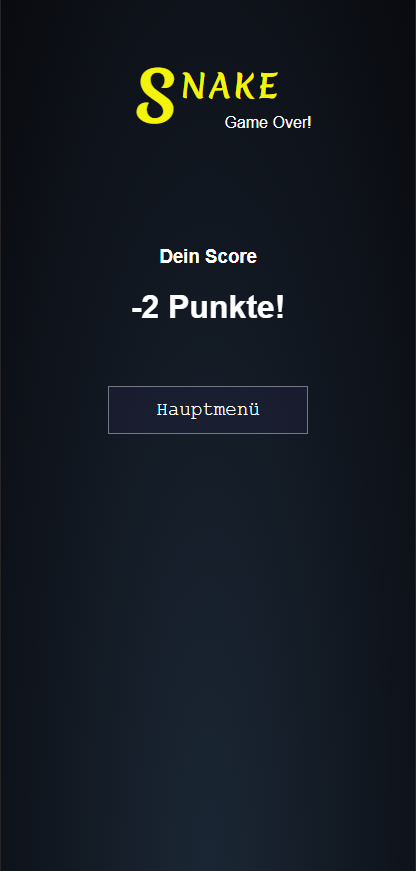
\includegraphics[width=\linewidth]{Abbildungen/Snake_Gameover.png}
      \caption{Snake Website Game Over Score}
      \label{fig:gameover}
   \end{minipage}
\end{figure}

\newpage

\section{Quellenverzeichnis}
\begin{itemize}
\item test
\end{itemize}

\end{document}